\section{Details}

\subsection*{Name}
While your character's kin description in the previous chapter contains a list of common names, you are welcome to create your own.
For this, you can use the names in that list as a rough guideline to understand how their naming conventions usually works.

Also think about how your character obtained their name.
Each kin's section provides some information about how it's common for a member of your kin to obtain a name.
Consider if this applies to your character and think what your character thinks of their name.
Are they proud of it or do they dislike its origin or meaning?

\subsection*{Sex}
Most of the kins are genderless, and thus sex and gender don't really have relevance in most societies of Yuadrem.
If you choose to make a character of one of the gendered kins, keep in mind that their place in society will be generally unaffected.

With the exception of the qulbaba ird's feathers, your character's stats and characteristics are unaffected by their sex.

\subsection*{Height and Weight}
Based on their kin, you can decide your character's height and weight using the information in the Kins chapter.
You are encouraged to think of how your character's ability scores relate to these characteristics, or even how they may clash.

As in the PHB, you can roll randomly using the Random Height and Weight table.
The dice roll given in the Height Modifier column determines the character's extra height (in cm) beyond the base height.
Then, the dice roll given in the Weight Modifier column determines the character's extra weight (in kg) beyond the base weight.

\begin{DndTable}[width=\linewidth, header=Random Height and Weight]{lp{0.7cm}p{1.2cm}p{0.7cm}p{1.2cm}}
    \textbf{Kin} & \textbf{Base Height} & \textbf{Height Modifier} & \textbf{Base Weight} & \textbf{Weight Modifier} \\
    Gat               & 120  & 1d10 $\times$ 3  &  40  & 1d20 $\times$ 1   \\
    Treb Gat          & 160  & 1d10 $\times$ 4  &  90  & 1d10 $\times$ 3   \\
    Ird               & 170  & 1d10 $\times$ 3  &  40  & 1d10 $\times$ 1   \\
    Thulkraka Ird     & 170  & 1d10 $\times$ 3  &  60  & 1d20 $\times$ 1   \\
    Marset            &  70  & 1d10 $\times$ 3  &  18  &  1d4 $\times$ 1   \\
    Oth               & 130  & 1d10 $\times$ 5  &  40  & 1d10 $\times$ 1   \\
    Naenk             & \multicolumn{4}{l}{See Size in page \pageref{kin::naenk.size}} \\
    Tsanek            & 180  & 1d10 $\times$ 2  &  60  & 1d20 $\times$ 1   \\
    Tortle            & 150  & 1d10 $\times$ 3  & 200  & 1d20 $\times$ 3   \\
    Grung             &  75  & 1d10 $\times$ 3  &  18  &  1d4 $\times$ 1   \\
    Uman              & 150  & 1d10 $\times$ 4  &  50  & 1d10 $\times$ 3   \\
    Zaloth            & 150  & 1d10 $\times$ 3  & < 1  & -                 \\
    Quies Operative   & 180  & 1d10 $\times$ 5  &  70  & 1d20 $\times$ 4   \\
    Quies Juggernaut  & 180  & 1d10 $\times$ 5  & 200  & 1d10 $\times$ 3   \\
    Quies Slag Worker & 180  & 1d10 $\times$ 5  & 250  & 1d10 $\times$ 5
\end{DndTable}

\subsection*{Physical Characteristics}
Apart from what you've already defined, you also choose your character's age and eye, hair, and skin color.
Some characteristics specific to your character's kin are also customizable, like a gat's horns or an ird's feather patterns.

To help set apart your character from the rest, consider also giving them an unusual or memorable physical characteristic, such as a scar, a limp, or a tattoo.
Think about how your character acquired such a feature and the story they might tell to explain it.

\subsection*{Qualar}
Most people keep their qualars hidden and unadulterated.
Some, however, enjoy carving messages or drawings into theirs, so as to enjoy themselves or to be remembered by the next carrier of the bone artifact.
A few even cut small dents into it to place gems or crystal windows into the tarry liquid hidden within.

Bonecarvers capable of crafting artificial qualars usually cut them into a specific design so that people know who made them.
These designs can take many forms, like simple geometrical shapes to fine trinkets with intricate shapes.
It is usual that these qualars are more expensive than the ones made by Ctereth, and the finest ones are usually reserved only for the elite.

You are free to choose a qualar that makes sense for your character within reason.
Also consider the relation your character has with their qualar.
Perhaps they treasure it as a reminder of a home now abandoned, or maybe they want to exchange it in the first available opportunity.

\subsection*{Tidal Alignment}
To define your character's moral compass and the way they interact with the world, define one or two dominant tides for them.
The phenomenon of the tides is described in page \pageref{ssec::tides}.

Examples of people aligned to each tide follow.

\subparagraph{Blue Tide} A philosopher obsessed with the pursuit of enlightenment.
A monk seeking wisdom to pass off to their school.
A shaman making decisions for their tribe using both reason and mysticism.

\subparagraph{Red Tide} An artist looking for passionate experiences to portray.
An adventurer defying dangers in search of action and emotion.
A crusader on a zealous quest for their divinity of choice.

\subparagraph{Silver Tide} A ranger traversing an unexplored forest to leave a mark on history.
A bard seeking to influence others with their music.
A knight performing glorious deeds to acquire fame.

\subparagraph{Indigo Tide} A congressperson writing laws to improve equity in their nation.
A judge executing impartial justice to improve society as a whole.
A tyrant governing under the hood of the greater good.

\subparagraph{Gold Tide} A philanthropist aiding communities with their wealth.
A crime lord who cares for their community for their own gain.
A priest aiding the locals to gain favor from their god.

When defining your character's tidal alignment, always remember that the tides are associated to action, not intention.
Even if your character is merely seeking power, if to attain it they perform noble actions for a faction they will still improve their alignment with the gold tide.

\begin{table*}[b]%
    \begin{DndTable}[width=\linewidth]{X}
        \centering
        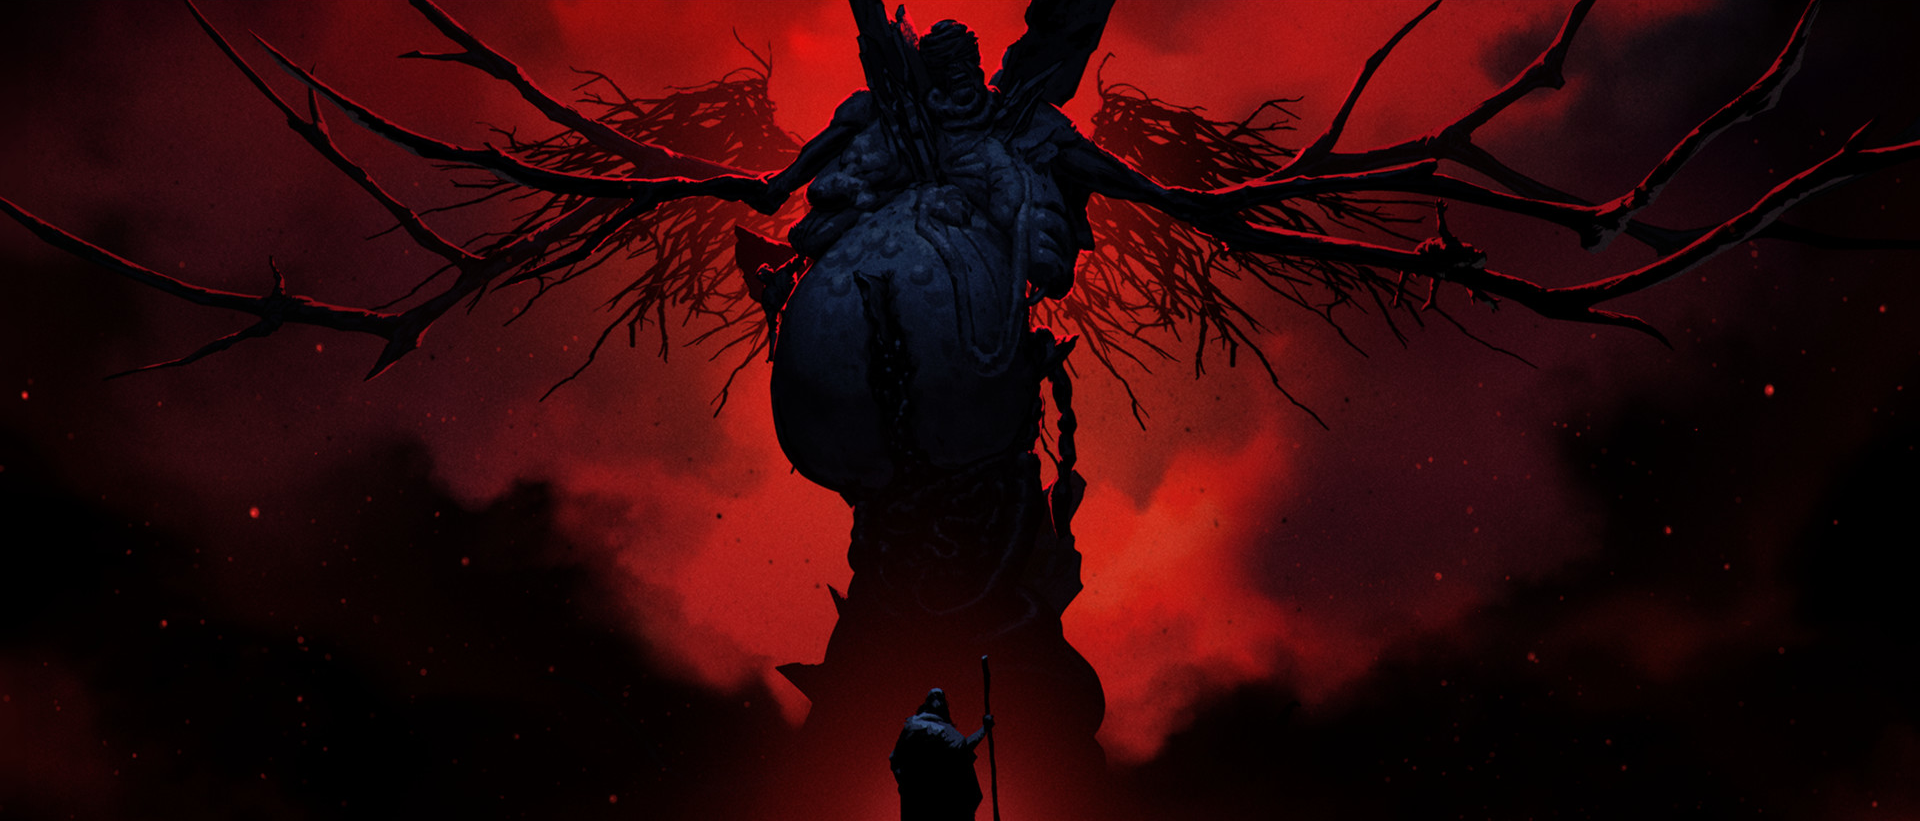
\includegraphics[width=0.95\textwidth]{05background/img/tidal_sway_rendition.png} \
        \centering \large{\textbf{Artist's Rendition of The Sorrow.}}
    \end{DndTable}
\end{table*}

\subsection*{Personal Characteristics}
For additional personal characteristics, you can follow the guidelines in pages 123 and 124 in the PHB.
You are not limited however to personality traits, ideals, bonds, and flaws.
You can flavor things as you see fit, adding attributes such as prides, dark secrets, flairs, etc.

Your character might take pride in their cooking even if they're not a professional chef.
Or they may have stolen an ancient family artifact before leaving home for adventure, claiming to have inherited it normally.
They may also be a particularly good juggler, and tend to juggle with stones when bored in a social situation.

Your character sheet includes an area to write your character's personal characteristics, but you are welcome to use additional sheets if your you need more space.
As advice, it's a good idea to put at least as much thought into your character's characteristics as you put into their appearance.
